% Options for packages loaded elsewhere
\PassOptionsToPackage{unicode}{hyperref}
\PassOptionsToPackage{hyphens}{url}
\PassOptionsToPackage{dvipsnames,svgnames,x11names}{xcolor}
\documentclass[
  11pt,
]{article}
\usepackage{xcolor}
\usepackage[margin=1in]{geometry}
\usepackage{amsmath,amssymb}
\setcounter{secnumdepth}{-\maxdimen} % remove section numbering
\usepackage{iftex}
\ifPDFTeX
  \usepackage[T1]{fontenc}
  \usepackage[utf8]{inputenc}
  \usepackage{textcomp} % provide euro and other symbols
\else % if luatex or xetex
  \usepackage{unicode-math} % this also loads fontspec
  \defaultfontfeatures{Scale=MatchLowercase}
  \defaultfontfeatures[\rmfamily]{Ligatures=TeX,Scale=1}
\fi
\usepackage{lmodern}
\ifPDFTeX\else
  % xetex/luatex font selection
\fi
% Use upquote if available, for straight quotes in verbatim environments
\IfFileExists{upquote.sty}{\usepackage{upquote}}{}
\IfFileExists{microtype.sty}{% use microtype if available
  \usepackage[]{microtype}
  \UseMicrotypeSet[protrusion]{basicmath} % disable protrusion for tt fonts
}{}
\makeatletter
\@ifundefined{KOMAClassName}{% if non-KOMA class
  \IfFileExists{parskip.sty}{%
    \usepackage{parskip}
  }{% else
    \setlength{\parindent}{0pt}
    \setlength{\parskip}{6pt plus 2pt minus 1pt}}
}{% if KOMA class
  \KOMAoptions{parskip=half}}
\makeatother
\usepackage{longtable,booktabs,array}
\usepackage{caption}
\captionsetup[table]{skip=6pt}
\newcounter{none} % for unnumbered tables
\usepackage{calc} % for calculating minipage widths
% Correct order of tables after \paragraph or \subparagraph
\usepackage{etoolbox}
\makeatletter
\patchcmd\longtable{\par}{\if@noskipsec\mbox{}\fi\par}{}{}
\makeatother
\usepackage{graphicx}
\makeatletter
\newsavebox\pandoc@box
\newcommand*\pandocbounded[1]{% scales image to fit in text height/width
  \sbox\pandoc@box{#1}%
  \Gscale@div\@tempa{\textheight}{\dimexpr\ht\pandoc@box+\dp\pandoc@box\relax}%
  \Gscale@div\@tempb{\linewidth}{\wd\pandoc@box}%
  \ifdim\@tempb\p@<\@tempa\p@\let\@tempa\@tempb\fi% select the smaller of both
  \ifdim\@tempa\p@<\p@\scalebox{\@tempa}{\usebox\pandoc@box}%
  \else\usebox{\pandoc@box}%
  \fi%
}
% Set default figure placement to htbp
\def\fps@figure{htbp}
\makeatother
\setlength{\emergencystretch}{3em} % prevent overfull lines
\providecommand{\tightlist}{%
  \setlength{\itemsep}{0pt}\setlength{\parskip}{0pt}}

\usepackage{etoolbox}
\AtBeginEnvironment{longtable}{\small\setlength{\tabcolsep}{4pt}}
\setlength{\emergencystretch}{3em}
\usepackage{amssymb}
\usepackage{bookmark}
\IfFileExists{xurl.sty}{\usepackage{xurl}}{} % add URL line breaks if available
\urlstyle{same}
% fallback for those not using the hyperref driver hyperxmp:
\makeatletter
\@ifundefined{xmpquote}{\newcommand{\xmpquote}[1]{#1}}{}
\makeatother
\hypersetup{
  pdftitle={Shared Initialisation Confounds the LoRA Evidence for Universal Weight Subspaces},
  colorlinks=true,
  linkcolor={blue},
  filecolor={Maroon},
  citecolor={Blue},
  urlcolor={blue},
  pdfcreator={LaTeX via pandoc}}

\title{Shared Initialisation Confounds the LoRA Evidence for Universal
Weight Subspaces}
\author{Noah Persaud\\ Holdout Labs\\ \texttt{noah@holdoutlabs.ai}}
\date{October 11, 2026}

\begin{document}
\maketitle
\begin{abstract}
Kaushik et al.~(2026a; arXiv 2512.05117 v3) report that about 500 LoRA
adapters for Mistral-7B, each trained on a different task, share a
low-dimensional ``universal'' subspace, with ``most information
concentrated in 16 or fewer directions across all layers''. LoRA
initialises its down-projection A at random and its up-projection B at
zero, and A moves little in training. We therefore asked how much of
this structure comes from shared initialisation. On the adapters listed
in the paper's Table 10 (497 inferred to have been used for fitting;
including all 502 changes nothing material), 255 of 497 (51\%) form one
group whose A matrices are nearly identical across different tasks
(median pairwise cosine 0.90), consistent with a reused random
initialisation. Across the whole public collection the fraction is 38\%,
so the paper's set is enriched for it. In the paper's analysis, this
group puts 86--90\% of A's variance in 16 directions; the 242 adapters
outside it put 2--5\%, close to independent random matrices at the same
sample size (1.6\%). A simulated collection with the same grouping and
no training at all shows the same rank-16 knee. The effect survives a
factorisation-invariant analysis of \(\Delta W = BA\) on the input side.
The output side behaves differently: it shows shared structure that is
present in both inferred groups, exceeds a null that preserves each
adapter's singular values in every layer we examined, and outside the
first layer is little reduced by removing the base model's dominant
weight directions. In a controlled experiment on Qwen2.5-0.5B-Instruct,
the same ten tasks show the rank-16 A subspace when they share an
initialisation and the random level when they do not; a rank-16 basis
fitted on other tasks captures little of a held-out task's update, and
projecting one side at a time shows that within a shared initialisation
the loss comes mainly from the fitted output basis, for factor-based and
factorisation-invariant bases alike. Although the fitted output bases
retain little update energy, they preserve partial performance on two of
the nine learned tasks (paraphrase and concise rewriting). We conclude
that the input-side (A) evidence for a universal LoRA subspace is
largely an initialisation artefact, while a weaker, genuinely shared
output-side structure deserves separate study. We recommend that
analyses of adapter collections report seeds, group by inferred
initialisation, use factorisation-invariant statistics and compare
against strength-matched nulls.
\end{abstract}

\section{1. Introduction}\label{introduction}

The Universal Weight Subspace Hypothesis (Kaushik et al., 2026a, arXiv
2512.05117; we review v3, dated 2026-10-05) proposes that neural
networks converge to shared spectral subspaces ``regardless of
initialization, task, or domain''. One line of evidence is a collection
of LoRA adapters (Hu et al., 2022) for Mistral-7B-Instruct-v0.2, each
trained on a Natural Instructions task (Wang et al., 2022) and released
by Br\"{u}el-Gabrielsson et al.~(2025). The headline for this collection,
``most information concentrated in 16 or fewer directions across all
layers'', is in the caption of the paper's Figure 4. For each layer, the
paper concatenates the rank vectors of all adapters into a
\(500r \times d\) matrix, separately for the factors A and B, subtracts
the feature-wise mean and extracts principal directions (Appendix B.5);
the orientation of A and B follows from this shape. The paper
acknowledges that ``the LoRA factorization is not unique'', notes that
``a gauge-invariant alternative would perform the same analysis directly
on \(\Delta W\)'', and states that its analysis ``characterizes
recurring structure in the learned and stored LoRA parameterization,
rather than a gauge-invariant property of the equivalent full update
\(\Delta W = BA\)''. We found no seed information and no random-matrix
baseline for this analysis anywhere in the paper.

Two facts make initialisation a candidate explanation. First, PEFT
initialises A with a Kaiming-uniform draw from the global random
generator, so adapters created with the same seed and configuration
start from an identical A, provided the generator is in the same state,
with the same sequence of earlier draws, when A is drawn. Second, A
moves little in training. In our own controlled runs on
Qwen2.5-0.5B-Instruct and Llama-3.2-1B-Instruct (40 runs;
\href{https://github.com/P1ayer-1/Adaptation-Geometry/blob/35296cb03172d6fee33797979a4e4e5d03e90318/docs/dev_scale_report.md}{\texttt{dev\_\allowbreak{}scale\_\allowbreak{}report.md}}),
\(\|A - A_0\|_F / \|A_0\|_F\) was 0.04--0.22, and under a shared seed
the input subspaces of unrelated tasks overlapped by 97--99\%. If many
adapters in a collection share an initialisation, the stacked A matrix
contains the same r = 16 random vectors many times, and PCA finds about
16 dominant directions whatever the tasks.

Contributions:

\begin{enumerate}
\def\labelenumi{\arabic{enumi}.}
\tightlist
\item
  On the paper's adapter list (the inferred fitting set, Section 2), we
  identify one large group of adapters with a common,
  initialisation-like A (51\%), robust to the grouping threshold and
  identical in all layers examined (Section 3.1).
\item
  A matched comparison, size-matched random nulls and a no-training
  simulation show that the rank-16 A spectrum comes from this group
  (Section 3.2, Figure 1).
\item
  A crossed task \texorpdfstring{\ensuremath{\times}}{x} initialisation experiment on Qwen2.5-0.5B-Instruct
  separates seed from task directly, and one-sided projections locate
  where a fitted subspace fails to carry a new task (Section 3.3).
\item
  A factorisation-invariant analysis with strength-matched nulls
  separates what the shared initialisation explains (input side) from
  genuinely shared structure (output side), and tests how much of the
  latter is the base model's dominant directions (Sections 3.4--3.5).
\item
  The same grouping affects joint-basis compression of this collection
  (Section 3.6).
\end{enumerate}

We do not test the paper's results on fully trained models (ViTs,
ResNets), which do not involve LoRA initialisation.

\section{2. Setup}\label{setup}

\textbf{Adapters.} Table 10 of v3 lists 502 adapters
\texttt{Lots-\allowbreak{}of-\allowbreak{}LoRAs/\allowbreak{}Mistral-\allowbreak{}7B-\allowbreak{}Instruct-\allowbreak{}v0.2-\allowbreak{}4b-\allowbreak{}r16-\allowbreak{}taskNNN} (all
present in the public collection of 904 rank-16 adapters). Five are
coloured as out-of-distribution evaluation models. We infer from the
colouring that the other 497 were used to fit the subspace and call them
the \emph{inferred fitting set}; ``the paper's set'' below means this
set. The split is not confirmed by the authors, so Section 3.1 reports
the sensitivity to including all 502. Each adapter adapts the q, k and v
projections of all 32 layers with rank r = 16 and scaling
\(\alpha/r = 2\) (constant, so it cancels in every normalised statistic
below). A is \(r \times d_{\text{in}}\) (\(d_{\text{in}} = 4{,}096\)); B
is \(d_{\text{out}} \times r\), with \(d_{\text{out}} = 4{,}096\) for q
and 1,024 for k and v (grouped-query attention). A \textbf{slot} is one
(layer, projection) pair; we analyse 15 slots: layers 0, 8, 16, 24, 31 \texorpdfstring{\ensuremath{\times}}{x}
q, k, v.

\textbf{Paper-style spectrum.} For a set of N adapters, stack the r rows
of each A (or the r columns of each B) into an \((N r) \times d\)
matrix, centre feature-wise and compute eigenvalues. \textbf{Top-16
share} is the fraction of variance in the 16 largest components;
\textbf{k90} is the number of components needed for 90\% of the
variance.

\textbf{Factorisation-invariant spectra.} Writing
\(\Delta W_i = B_i A_i\), we use the uncentred operators
\(C_{\text{in}} = \sum_i \Delta W_i^\top \Delta W_i\) and
\(C_{\text{out}} = \sum_i \Delta W_i \Delta W_i^\top\), whose spectra do
not depend on how \(\Delta W_i\) is split into factors (computed from
each adapter's compact SVD via QR of \(B\) and \(A^\top\)). We report
their top-16 share. These are one-sided measures of update energy, not
PCA over vectorised updates.

\textbf{Nulls.} (i) \emph{Size-matched independent initialisations}: N
fresh Kaiming-uniform A matrices, 10 repeats. (ii)
\emph{Strength-matched}: every adapter keeps its singular values and
gets random orthonormal singular vectors, 10 repeats; this tests
orientation given strength. (iii) \emph{Unit-norm} versions of the real
data and null (every \(\Delta W_i\) scaled to \(\|\Delta W_i\|_F = 1\)),
which remove differences in adapter norm and keep only within-adapter
anisotropy.

\textbf{Inferred groups.} Adapters are linked when the cosine similarity
of their layer-0 q\_proj A matrices exceeds 0.5; groups are connected
components. We call the large component the \emph{inferred
shared-initialisation group} and the rest \emph{singletons}. These are
inferences from A, not recovered training histories.

\section{3. Results}\label{results}

\subsection{3.1 One large group shares an initialisation-like
A}\label{one-large-group-shares-an-initialisation-like-a}

On the paper's 497 adapters the grouping yields one group of 255 (51\%)
and 242 singletons; no other multi-member groups. Within the group,
pairwise cosine of layer-0 q\_proj A has minimum 0.55, 10th percentile
0.78 and median 0.90. Between groups, 98\% of cosines lie within \ensuremath{\pm}0.010
and the largest is 0.044. The partition is identical for every threshold
from 0.15 to 0.6, and the same partition is obtained independently from
each of the 15 slots.

\emph{Sensitivity to the inferred split.} Including the five
out-of-distribution adapters (all 502) leaves the partition unchanged:
none of the five joins the group, which stays at 255 members, and the
other 247 adapters are singletons. The full-set top-16 share of A
changes by \ensuremath{-}0.004 to \ensuremath{-}0.005 in every slot (0.43--0.45; k90
1,632--1,759).

The group's mean A behaves like an initialisation plus a small averaged
change. Its kurtosis is 1.80--1.84 across slots (1.80 for a uniform
distribution, 3.0 for a Gaussian); its element standard deviation is
0.00901--0.00908 (0.00902 for PEFT's \(U(-1/64, 1/64)\)); its largest
entries reach 0.016--0.020, slightly beyond the uniform bound of 0.0156,
as expected if the mean includes some learned change. Individual
adapters lie a median 0.22--0.32 (10th-90th percentile 0.06--0.65) of
the mean's norm away from it. These are distances from the trained group
mean, not from the initialisation, and they bound neither an individual
adapter's movement nor the median movement. Only an aggregate statement
holds: since \(\sum_i \|A_i - m\|^2 \le \sum_i \|A_i - c\|^2\) for the
mean m and any common point c, the root-mean-square distance from the
mean, 0.33--0.39 of the mean's norm across slots, cannot exceed the
root-mean-square distance from the shared initialisation, measured in
the same units.

\textbf{Collection-wide.} Over all 904 rank-16 adapters, 342 (38\%)
belong to the group. The fraction varies with task number (25--51\%
across ranges). The paper's set (51\%) is enriched relative to a random
500 (39\%), the lowest-numbered 500 (44\%) and the whole collection
(38\%), and the top-16 share of layer-0 q\_proj A tracks the group
fraction across these sets (0.45, 0.34, 0.38, 0.32).

The model cards and \texttt{adapter\_\allowbreak{}config.json} files contain no seed
and no evaluation results. Seed 42 and 14 other common seeds did not
match the group mean within the first 67 million draws of PyTorch's CPU
generator, and seeds 0--199 did not match at the first six draw
positions; the generator may have been advanced by other code, or the
adapters created on a GPU. Nothing below depends on the seed.

\subsection{3.2 The rank-16 A spectrum comes from the
group}\label{the-rank-16-a-spectrum-comes-from-the-group}

{\def\LTcaptype{none} % do not increment counter
\begin{longtable}[]{@{}
  >{\raggedright\arraybackslash}p{(\linewidth - 4\tabcolsep) * \real{0.3256}}
  >{\raggedright\arraybackslash}p{(\linewidth - 4\tabcolsep) * \real{0.4186}}
  >{\raggedright\arraybackslash}p{(\linewidth - 4\tabcolsep) * \real{0.2558}}@{}}
\toprule\noalign{}
\begin{minipage}[b]{\linewidth}\raggedright
Paper-style A spectrum (15 slots)
\end{minipage} & \begin{minipage}[b]{\linewidth}\raggedright
Top-16 share
\end{minipage} & \begin{minipage}[b]{\linewidth}\raggedright
k90
\end{minipage} \\
\midrule\noalign{}
\endhead
\bottomrule\noalign{}
\endlastfoot
Paper's set (497 adapters) & 0.44\nobreakdash--0.46 & 1,610\nobreakdash--1,738 \\
Same grouping, pure initialisations, no training & 0.51 & --- \\
Same grouping, initialisations + random movement of the measured size &
0.46\nobreakdash--0.48 & --- \\
Shared-initialisation group (242 of 255) & 0.86\nobreakdash--0.90 & 16\nobreakdash--90 \\
Singletons (242) & 0.021\nobreakdash--0.052 & 1,980\nobreakdash--2,003 \\
Independent random initialisations (242, 10 repeats) & 0.016 (sd
\textless{} 0.001) & --- \\
\end{longtable}
}

(Rank caps: 4,096 for the full set; 3,871 for 242 adapters after
centring.)

The paper's set shows a sharp knee at exactly the LoRA rank (Figure 1).
A collection with the same grouping and no training at all reproduces
the knee, and adding random movement of the measured size brings the
top-16 share to within 0.02--0.04 of the real value. Under row stacking,
the top-16 share of such a collection is roughly the shared fraction
times the share of each group member's variance carried by the common A,
which is why it tracks the group fraction (Section 3.1). Singletons are
1.3--3.3 times the size-matched random level, highest in layer 0
(0.036--0.052), so they are close to, but not exactly, random. The
rank-16 concentration is absent among them.

For B, the group and the singletons agree to within 0.015 in every slot
(top-16 share 0.11--0.56), so B has similar spectra in both groups.

\begin{figure}
\centering
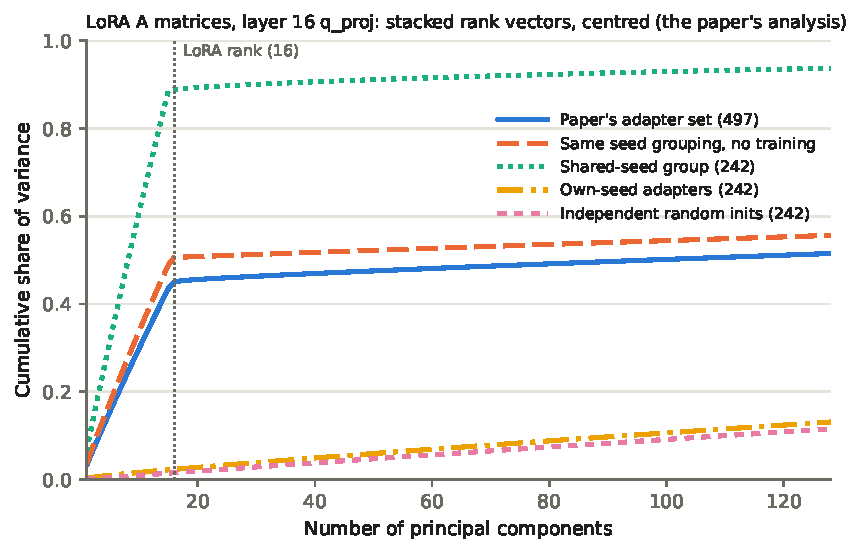
\includegraphics[width=0.8\linewidth,height=\textheight,keepaspectratio,alt={Cumulative
variance of the paper-style A spectrum, layer 16 q\_proj. The paper's
set and a no-training simulation with the same grouping both jump at the
LoRA rank; adapters outside the group are close to independent random
matrices.}]{figures/figure1_spectrum.pdf}
\caption{Cumulative variance of the paper-style A spectrum, layer 16
q\_proj. The paper's set and a no-training simulation with the same
grouping both jump at the LoRA rank; adapters outside the group are
close to independent random matrices.}
\end{figure}

\subsection{3.3 Crossed task \texorpdfstring{\ensuremath{\times}}{x} initialisation
experiment}\label{crossed-task-initialisation-experiment}

To separate initialisation from task directly, we trained the same 10
tasks (our synthetic panel: hidden-rule sentiment, NLI, paraphrase, JSON
extraction, concise and verbose rewriting, Python, arithmetic, clinical
extraction, formatting) on Qwen2.5-0.5B-Instruct, rank 16 on all seven
projection types (168 modules), with identical data, optimiser and early
stopping, under two regimes: \textbf{shared}, one random A per seed used
by every task (two seeds, so two shared initialisations), and
\textbf{independent}, a separate random A per task and seed. A hardware
check retrained four independent runs on a different GPU (RTX 3080 vs
A100) from the same initialisation: \(\Delta W\) cosine 0.88--0.94 and A
cosine \ensuremath{\ge} 0.997, so training is reproducible across machines.

{\def\LTcaptype{none} % do not increment counter
\begin{longtable}[]{@{}
  >{\raggedright\arraybackslash}p{(\linewidth - 2\tabcolsep) * \real{0.6364}}
  >{\raggedright\arraybackslash}p{(\linewidth - 2\tabcolsep) * \real{0.3636}}@{}}
\toprule\noalign{}
\begin{minipage}[b]{\linewidth}\raggedright
Paper-style A spectrum, 10 adapters per group
\end{minipage} & \begin{minipage}[b]{\linewidth}\raggedright
Top-16 share (median over 168 modules)
\end{minipage} \\
\midrule\noalign{}
\endhead
\bottomrule\noalign{}
\endlastfoot
Shared initialisation (each of the two groups) & 0.99 \\
Both shared groups pooled (20 adapters) & 0.59 \\
Independent initialisations & 0.18 \\
Independent random matrices, same N & 0.18 \\
\end{longtable}
}

With everything else fixed, the rank-16 subspace appears when tasks
share an initialisation, splits into two subspaces when two
initialisations are pooled, and is at the random level when
initialisations are independent.

\textbf{Projection onto bases fitted on other tasks.} For each held-out
task we fitted rank-16 input and output bases on the other nine tasks
and projected the held-out adapter onto them, on both sides
(\(\Delta W' = U U^\top B A V V^\top\)), on the input side only
(\(\Delta W' = B A V V^\top\), keeping the adapter's own output
directions) or on the output side only (\(\Delta W' = U U^\top B A\),
keeping its own input directions). We fitted the bases in three ways.
\emph{Invariant} bases are the top eigenvectors of the uncentred
operators \(C_{\text{in}} = \sum \Delta W^\top \Delta W\) and
\(C_{\text{out}} = \sum \Delta W \Delta W^\top\) over the nine tasks
(Section 2); they do not depend on how each update is split into B and
A. \emph{Centred factor} bases follow the paper's convention: the top
principal directions of the stacked raw A rows (V) and B columns (U)
after subtracting the feature-wise mean. \emph{Uncentred factor} bases
are the top singular vectors of the same stacks without centring. Each
shared initialisation was held out in turn, with bases from the same and
from the other initialisation; the independent group was held out
against itself.

{\def\LTcaptype{none} % do not increment counter
\begin{longtable}[]{@{}
  >{\raggedright\arraybackslash}p{(\linewidth - 6\tabcolsep) * \real{0.4667}}
  >{\raggedright\arraybackslash}p{(\linewidth - 6\tabcolsep) * \real{0.1667}}
  >{\raggedright\arraybackslash}p{(\linewidth - 6\tabcolsep) * \real{0.2000}}
  >{\raggedright\arraybackslash}p{(\linewidth - 6\tabcolsep) * \real{0.1667}}@{}}
\toprule\noalign{}
\begin{minipage}[b]{\linewidth}\raggedright
Held-out adapter, basis from other tasks
\end{minipage} & \begin{minipage}[b]{\linewidth}\raggedright
Input side only
\end{minipage} & \begin{minipage}[b]{\linewidth}\raggedright
Output side only
\end{minipage} & \begin{minipage}[b]{\linewidth}\raggedright
Both sides
\end{minipage} \\
\midrule\noalign{}
\endhead
\bottomrule\noalign{}
\endlastfoot
Init 0, same init & 0.924 & 0.073 & 0.068 \\
Init 1, same init & 0.925 & 0.089 & 0.080 \\
Init 0, other init & 0.018 & 0.072 & 0.002 \\
Init 1, other init & 0.018 & 0.086 & 0.002 \\
Independent & 0.021 & 0.084 & 0.002 \\
\end{longtable}
}

(Invariant bases; share of the held-out \(\|\Delta W\|_F^2\) captured,
median over 10 tasks. Ranges over tasks and all three bases: input side
with the same initialisation 0.77--0.99, otherwise 0.016--0.023; output
side 0.033--0.130; both sides with the same initialisation 0.027--0.118,
otherwise 0.001--0.004. Appendix B gives the factor bases, whose medians
differ from these by at most 0.037.) With uncentred factor bases from
crossed\_eval.py and initialisation 0 held out, adding the held-out task
itself, trained from the other initialisation, to the basis raises the
two-sided share only to 0.006 (0.002--0.011).

We scored the projected adapters of all ten tasks with invariant bases,
and of four tasks with centred factor bases (Appendix A explains the
choice of four).

{\def\LTcaptype{none} % do not increment counter
\begin{longtable}[]{@{}
  >{\raggedright\arraybackslash}p{(\linewidth - 14\tabcolsep) * \real{0.1647}}
  >{\raggedright\arraybackslash}p{(\linewidth - 14\tabcolsep) * \real{0.0588}}
  >{\raggedright\arraybackslash}p{(\linewidth - 14\tabcolsep) * \real{0.1294}}
  >{\raggedright\arraybackslash}p{(\linewidth - 14\tabcolsep) * \real{0.1294}}
  >{\raggedright\arraybackslash}p{(\linewidth - 14\tabcolsep) * \real{0.1294}}
  >{\raggedright\arraybackslash}p{(\linewidth - 14\tabcolsep) * \real{0.1294}}
  >{\raggedright\arraybackslash}p{(\linewidth - 14\tabcolsep) * \real{0.1294}}
  >{\raggedright\arraybackslash}p{(\linewidth - 14\tabcolsep) * \real{0.1294}}@{}}
\toprule\noalign{}
\begin{minipage}[b]{\linewidth}\raggedright
Task
\end{minipage} & \begin{minipage}[b]{\linewidth}\raggedright
Base model
\end{minipage} & \begin{minipage}[b]{\linewidth}\raggedright
Direct adapters
\end{minipage} & \begin{minipage}[b]{\linewidth}\raggedright
Input only, same init
\end{minipage} & \begin{minipage}[b]{\linewidth}\raggedright
Output only, same init
\end{minipage} & \begin{minipage}[b]{\linewidth}\raggedright
Both, same init
\end{minipage} & \begin{minipage}[b]{\linewidth}\raggedright
Both, other init
\end{minipage} & \begin{minipage}[b]{\linewidth}\raggedright
Both, independent
\end{minipage} \\
\midrule\noalign{}
\endhead
\bottomrule\noalign{}
\endlastfoot
Hidden-rule sentiment & 0.485 & 0.455\nobreakdash--0.515 & 0.470\nobreakdash--0.505 & 0.485 &
0.485 & 0.485 & 0.485 \\
NLI & 0.360 & 0.755\nobreakdash--0.760 & 0.625\nobreakdash--0.695 & 0.330\nobreakdash--0.350 & 0.315\nobreakdash--0.330
& 0.360 & 0.360 \\
Paraphrase & 0.650 & 0.975\nobreakdash--1.000 & 0.955\nobreakdash--0.995 & 0.715\nobreakdash--0.720 &
0.705\nobreakdash--0.715 & 0.650 & 0.655 \\
JSON extraction & 0.000 & 1.000 & 0.755\nobreakdash--0.865 & 0.000 & 0.000 & 0.000 &
0.000 \\
Concise rewriting & 0.000 & 0.855\nobreakdash--0.925 & 0.885\nobreakdash--0.910 & 0.395\nobreakdash--0.460 &
0.395\nobreakdash--0.410 & 0.000 & 0.000 \\
Verbose rewriting & 0.000 & 0.925\nobreakdash--0.935 & 0.875\nobreakdash--0.885 & 0.000 & 0.000
& 0.000 & 0.000 \\
Python & 0.035 & 0.970\nobreakdash--1.000 & 0.995\nobreakdash--1.000 & 0.020\nobreakdash--0.025 & 0.170 &
0.040\nobreakdash--0.045 & 0.060 \\
Arithmetic & 0.000 & 0.895\nobreakdash--0.915 & 0.900\nobreakdash--0.915 & 0.000 & 0.000\nobreakdash--0.010
& 0.000 & 0.000 \\
Clinical extraction & 0.000 & 1.000 & 0.865\nobreakdash--0.880 & 0.000 & 0.000 &
0.000 & 0.000 \\
Formatting & 0.000 & 0.910\nobreakdash--0.980 & 0.395\nobreakdash--0.480 & 0.000 & 0.000 & 0.000
& 0.000 \\
\end{longtable}
}

(Invariant bases; test sets of n = 200. Each cell gives the range over
the held-out conditions it pools: ``same init'' pools initialisation 0
and 1 held out against their own group, ``other init'' pools each held
out against the other group. Direct adapters are those of the three
groups. All scores come from one run on the same GPU, base model
included. Appendix B gives every condition and the centred factor
bases.)

The following points concern the fitted rank-16 bases, not every basis
that could be built from the nine tasks or one of higher rank.

\begin{enumerate}
\def\labelenumi{\arabic{enumi}.}
\tightlist
\item
  \emph{Hidden-rule sentiment is uninformative.} Its direct adapters
  score at the base model's level (0.455--0.515 against 0.485), so the
  task was not learned and is left out below.
\item
  \emph{The fitted input basis is the initialisation's.} With the same
  initialisation, the input-only projection keeps about 90\% of the
  update's energy and most of six of the nine learned tasks (0.865--1.00
  on paraphrase, concise and verbose rewriting, Python, arithmetic and
  clinical extraction), with partial retention on JSON extraction
  (0.755--0.865), NLI (0.625--0.695) and formatting (0.395--0.48). With
  a basis from another or an independent initialisation it keeps about
  2\% of the energy, and every learned task returns to within 0.03 of
  the base model, except concise rewriting with the independent basis
  (0.095).
\item
  \emph{The fitted output basis captures 7--9\% of a held-out update's
  energy in every condition.} The output-only projection removes all or
  nearly all of the effect on seven of the nine learned tasks: NLI, JSON
  extraction, verbose rewriting, Python, arithmetic, clinical extraction
  and formatting score within 0.04 of the base model, most at or below
  it. Two tasks keep part of it in every condition, including bases from
  another initialisation: paraphrase (0.71--0.73 against 0.65) and
  concise rewriting (0.375--0.46 against 0, where the direct adapters
  reach 0.855--0.925). Within one initialisation, then, the two-sided
  loss comes mainly from the output side. The exceptions show that, in
  this model, output directions shared across tasks can carry part of a
  task; they do not establish what the residual output-side structure of
  the Mistral collection (Sections 3.4--3.5) represents.
\item
  \emph{Two-sided projection with the same initialisation leaves most
  learned tasks near the base model.} NLI, JSON extraction, verbose
  rewriting, arithmetic, clinical extraction and formatting score
  0--0.01 above the base model or below it. Three tasks keep a partial
  effect: concise rewriting (0.395--0.41), Python (0.17 against 0.035;
  paired \(p \le 3 \times 10^{-5}\)) and paraphrase (0.705--0.715
  against 0.65; paired differences 0.055--0.065, exact McNemar p =
  0.019--0.052). With a basis from another or an independent
  initialisation, the two-sided projection scores within 0.025 of the
  base model on every task, and no difference is significant at p
  \textless{} 0.05.
\item
  \emph{Centred factor bases give the same pattern.} On the four tasks
  scored with both, the centred factor bases keep somewhat less of JSON
  and clinical extraction on the input side (0.675--0.81 against
  0.755--0.88) and otherwise agree with the invariant bases to within
  0.03; median captured shares differ by at most 0.037. These results
  are therefore not an artefact of fitting bases to the raw factors.
\end{enumerate}

The experiment covers two shared initialisations, each held out in turn,
one independent group and one training run per task and initialisation.
It uses a small model and synthetic tasks, so it shows the mechanism
rather than replicating the paper. The paper's own held-out test also
projects held-out adapters onto the fitted subspace, with ``analytically
reconstructed'' coefficients (its Section 4 and Appendix B.7). There the
subspace is fitted on up to 450 adapters with an unstated number of
components, and nine held-out tasks reach Rouge-L 72.3 against 73.7 for
the original adapters (its Table 17). All nine are singletons under our
grouping, so their input sides do not share the group's initialisation;
four of them are in the set we infer as the fitting set of Table 10, so
B.7 uses a different split. The paper does not report the base model's
score on these tasks. Its stated 19-fold memory saving would be
consistent with roughly 140 components per factor if each adapter's
coefficients are stored densely, about nine times our rank 16. Our
rank-16 projections from nine tasks therefore test a much smaller basis
and do not contradict that result.

\subsection{3.4 Factorisation-invariant updates: input side and output
side
differ}\label{factorisation-invariant-updates-input-side-and-output-side-differ}

{\def\LTcaptype{none} % do not increment counter
\begin{longtable}[]{@{}
  >{\raggedright\arraybackslash}p{(\linewidth - 10\tabcolsep) * \real{0.2029}}
  >{\raggedright\arraybackslash}p{(\linewidth - 10\tabcolsep) * \real{0.1304}}
  >{\raggedright\arraybackslash}p{(\linewidth - 10\tabcolsep) * \real{0.1449}}
  >{\raggedright\arraybackslash}p{(\linewidth - 10\tabcolsep) * \real{0.2319}}
  >{\raggedright\arraybackslash}p{(\linewidth - 10\tabcolsep) * \real{0.1594}}
  >{\raggedright\arraybackslash}p{(\linewidth - 10\tabcolsep) * \real{0.1304}}@{}}
\toprule\noalign{}
\begin{minipage}[b]{\linewidth}\raggedright
Top-16 share (uncentred, 15 slots)
\end{minipage} & \begin{minipage}[b]{\linewidth}\raggedright
Group
\end{minipage} & \begin{minipage}[b]{\linewidth}\raggedright
Singletons
\end{minipage} & \begin{minipage}[b]{\linewidth}\raggedright
Strength-matched null
\end{minipage} & \begin{minipage}[b]{\linewidth}\raggedright
Singletons, unit-norm
\end{minipage} & \begin{minipage}[b]{\linewidth}\raggedright
Null, unit-norm
\end{minipage} \\
\midrule\noalign{}
\endhead
\bottomrule\noalign{}
\endlastfoot
Input side, layer 0 & 0.60\nobreakdash--0.67 & 0.22\nobreakdash--0.37 & 0.12\nobreakdash--0.32 & 0.10\nobreakdash--0.14
& 0.05\nobreakdash--0.07 \\
Input side, layers 8\nobreakdash--31 & 0.53\nobreakdash--0.60 & 0.11\nobreakdash--0.24 & 0.10\nobreakdash--0.22 &
0.05\nobreakdash--0.11 & 0.05\nobreakdash--0.07 \\
Output side, layer 0 & 0.21\nobreakdash--0.60 & 0.19\nobreakdash--0.62 & 0.14\nobreakdash--0.32 & 0.14\nobreakdash--0.59
& 0.07\nobreakdash--0.09 \\
Output side, layers 8\nobreakdash--31 & 0.17\nobreakdash--0.33 & 0.15\nobreakdash--0.30 & 0.10\nobreakdash--0.23 &
0.12\nobreakdash--0.26 & 0.05\nobreakdash--0.09 \\
\end{longtable}
}

\emph{Stability.} Over 20 subsamples of 193 of the 242 singletons
(without replacement, fresh null each time), the singleton excess over
the strength-matched null is stable. Input side, layers 8--31:
0.002--0.020 (sd \ensuremath{\le} 0.001); output side, layers 8--31: 0.019--0.097 raw
(sd \ensuremath{\le} 0.005) and 0.049--0.183 unit-norm (sd \ensuremath{\le} 0.006); layer 0 output q
and k: 0.21 and 0.34 raw (sd 0.011).

\emph{Input side.} The group remains far more concentrated than the
singletons in the invariant analysis (0.53--0.67 against 0.11--0.37), so
the A-side result is not an artefact of analysing the stored factors.
Outside layer 0, singletons exceed the strength-matched null by only
0.003--0.022 (unit-norm: up to 0.04). Layer 0 shows more (0.034--0.103).

\emph{Output side.} Group and singletons are similar (0.17--0.60 against
0.15--0.62), so the output-side concentration is present in both
inferred groups and does not track the shared initialisation. Singletons
exceed the strength-matched null in every slot: by 0.019--0.106 outside
layer 0 and by 0.22 (q) and 0.36 (k) in layer 0 (v: 0.047). With
unit-norm updates the gap widens (0.12--0.26 against 0.05--0.09 outside
layer 0), so it is not produced by a few large adapters.

\emph{What the null contains.} Each \(\Delta W\) is effectively low-rank
(median participation ratio 2.1--5.6 across slots; the top singular
value carries a median 34--67\% of each update's energy), and adapter
norms vary widely (largest/median 2.7--7.8; 90th/10th percentile
5.9--9.3). These alone give top-16 shares of 0.10--0.32, so equal-weight
random baselines overstate how surprising the observed concentration is.

\subsection{3.5 How much of the remaining structure is the base
model?}\label{how-much-of-the-remaining-structure-is-the-base-model}

We compare the singletons' shared subspaces with the base weight's
singular subspaces, and recompute the excess over the null after
projecting out the base weight's top-128 directions from both the data
and the null.

{\def\LTcaptype{none} % do not increment counter
\begin{longtable}[]{@{}
  >{\raggedright\arraybackslash}p{(\linewidth - 4\tabcolsep) * \real{0.1867}}
  >{\raggedright\arraybackslash}p{(\linewidth - 4\tabcolsep) * \real{0.2667}}
  >{\raggedright\arraybackslash}p{(\linewidth - 4\tabcolsep) * \real{0.5467}}@{}}
\toprule\noalign{}
\begin{minipage}[b]{\linewidth}\raggedright
Singletons
\end{minipage} & \begin{minipage}[b]{\linewidth}\raggedright
Overlap with base top-16 (\texorpdfstring{\ensuremath{\times}}{x} chance)
\end{minipage} & \begin{minipage}[b]{\linewidth}\raggedright
Energy in base top-128 directions: data (null)
\end{minipage} \\
\midrule\noalign{}
\endhead
\bottomrule\noalign{}
\endlastfoot
Input, layer 0 q / k / v & 44\texorpdfstring{\ensuremath{\times}}{x} / 32\texorpdfstring{\ensuremath{\times}}{x} / 22\texorpdfstring{\ensuremath{\times}}{x} & 0.19 / 0.14 / 0.09
(0.03) \\
Input, layers 8\nobreakdash--31 & 0.7\nobreakdash--6.2\texorpdfstring{\ensuremath{\times}}{x} & 0.03\nobreakdash--0.06 (0.03) \\
Output, layer 0 q / k / v & 17.6\texorpdfstring{\ensuremath{\times}}{x} / 12.4\texorpdfstring{\ensuremath{\times}}{x} / 1.8\texorpdfstring{\ensuremath{\times}}{x} & 0.43 / 0.71 / 0.17
(0.03 / 0.13 / 0.13) \\
Output, layers 8\nobreakdash--31 & 0.8\nobreakdash--3.0\texorpdfstring{\ensuremath{\times}}{x} & q 0.05 (0.03); k, v 0.12\nobreakdash--0.14
(0.12\nobreakdash--0.13) \\
\end{longtable}
}

(Overlap is the mean \(\cos^2\) of principal angles between the two
16-dimensional subspaces; chance is \(16/d\). Energy is the share of the
stacked rows' squared norm inside the base directions; the null's share
equals the chance level \(k/d\).)

Projecting directions out changes the denominator of the top-16 share,
so we report the excess under two conventions. With a \emph{fixed
denominator}, the top-16 energy left after projection is divided by the
total energy before it. With a \emph{renormalised} share, it is divided
by the energy left after projection.

{\def\LTcaptype{none} % do not increment counter
\begin{longtable}[]{@{}
  >{\raggedright\arraybackslash}p{(\linewidth - 6\tabcolsep) * \real{0.1772}}
  >{\raggedright\arraybackslash}p{(\linewidth - 6\tabcolsep) * \real{0.2658}}
  >{\raggedright\arraybackslash}p{(\linewidth - 6\tabcolsep) * \real{0.2911}}
  >{\raggedright\arraybackslash}p{(\linewidth - 6\tabcolsep) * \real{0.2658}}@{}}
\toprule\noalign{}
\begin{minipage}[b]{\linewidth}\raggedright
Singletons, excess over null
\end{minipage} & \begin{minipage}[b]{\linewidth}\raggedright
Before
\end{minipage} & \begin{minipage}[b]{\linewidth}\raggedright
After removing base top-128, fixed denominator
\end{minipage} & \begin{minipage}[b]{\linewidth}\raggedright
After, renormalised
\end{minipage} \\
\midrule\noalign{}
\endhead
\bottomrule\noalign{}
\endlastfoot
Input, layer 0 q / k / v & 0.053 / 0.034 / 0.103 & \ensuremath{-}0.049 / \ensuremath{-}0.025 /
0.078 & 0.001 / 0.002 / 0.094 \\
Input, layers 8\nobreakdash--31 & 0.003\nobreakdash--0.022 & \ensuremath{-}0.004\nobreakdash--0.020 & 0.000\nobreakdash--0.021 \\
Output, layer 0 q / k / v & 0.220 / 0.361 / 0.046 & \ensuremath{-}0.028 / \ensuremath{-}0.111 /
0.033 & 0.177 / 0.146 / 0.048 \\
Output, layers 8\nobreakdash--31 & 0.019\nobreakdash--0.105 & 0.015\nobreakdash--0.100 & 0.018\nobreakdash--0.119 \\
\end{longtable}
}

(10 null repeats; the null is the strength-matched null of Section 2,
projected the same way.)

In layer 0 q and k the singletons put far more energy in the base
weight's top directions than the null does (on the output side of k,
71\% against 12.5\%). Removing those directions therefore takes more
energy from the data than from the null, and with a fixed denominator
the excess turns negative. With the renormalised share, the input excess
in layer 0 q and k disappears, and the output excess falls from 0.36 to
0.15 (k) and from 0.22 to 0.18 (q). The two conventions answer different
questions: how much of the original concentration survives, and how
concentrated the remainder is. Neither gives a percentage of the excess
``explained'' by the base weight, so we report both rather than a single
figure. In layer 0 the shared structure is strongly aligned with the
base weight's dominant directions on both sides.

Outside layer 0 the conventions agree. The singletons put roughly as
much energy in the base directions as the null (1.0--1.5 times on the
output side, 1.0--1.8 times on the input side), and the output excess
changes little under either convention. The output-side shared structure
outside layer 0 is therefore present in both inferred groups, above a
strength-matched null, and little reduced by removing base-weight
directions. We do not know what it is; candidates include directions
favoured by the training data format common to all Natural Instructions
tasks, and activation statistics that weight singular vectors do not
capture.

\textbf{Learned movement of A.} Within the group, A minus the group mean
is modestly more concentrated than a strength-matched null (top-16 share
0.09--0.30 against 0.07--0.17; largest in layer 0), so training moves A
in partly shared directions, but this is small next to the
initialisation.

\subsection{3.6 The grouping also affects
compression}\label{the-grouping-also-affects-compression}

Br\"{u}el-Gabrielsson et al.~(2025), who trained this collection, serve many
LoRAs by approximating each update as \(U \Sigma_i V^\top\) with shared
bases U, V (``joint diagonalization''). They report that ``multiple
clusters significantly aid performance for \(n \geq 100\)'' and
recommend choosing ``the minimal number of clusters that achieves a
reconstruction loss below 0.6''. They describe this loss in words, as
the mean relative reconstruction error of the product BA, without a
formula, so it is not stated whether it is squared. We re-implemented
JD-Full (updates normalised to unit Frobenius norm, as they do; 10
alternating iterations; no clustering) on 100-adapter sets, for 6 slots
(layers 0, 16, 31 \texorpdfstring{\ensuremath{\times}}{x} q, v). We report the mean relative squared Frobenius
error \(1 - \|U^\top \Delta W_i V\|_F^2\) per adapter. With unit-norm
updates this equals the pooled squared error ratio
\(\sum_i \|U \Sigma_i V^\top - \Delta W_i\|_F^2 / \sum_i \|\Delta W_i\|_F^2\)
bounded in their Theorem 1; it is comparable with their 0.6 threshold
only if that threshold is also squared.

{\def\LTcaptype{none} % do not increment counter
\begin{longtable}[]{@{}
  >{\raggedright\arraybackslash}p{(\linewidth - 8\tabcolsep) * \real{0.1000}}
  >{\raggedright\arraybackslash}p{(\linewidth - 8\tabcolsep) * \real{0.2250}}
  >{\raggedright\arraybackslash}p{(\linewidth - 8\tabcolsep) * \real{0.2250}}
  >{\raggedright\arraybackslash}p{(\linewidth - 8\tabcolsep) * \real{0.2250}}
  >{\raggedright\arraybackslash}p{(\linewidth - 8\tabcolsep) * \real{0.2250}}@{}}
\toprule\noalign{}
\begin{minipage}[b]{\linewidth}\raggedright
Rank
\end{minipage} & \begin{minipage}[b]{\linewidth}\raggedright
Group set
\end{minipage} & \begin{minipage}[b]{\linewidth}\raggedright
Singleton set
\end{minipage} & \begin{minipage}[b]{\linewidth}\raggedright
Mixed 50/50: group half
\end{minipage} & \begin{minipage}[b]{\linewidth}\raggedright
Mixed: singleton half
\end{minipage} \\
\midrule\noalign{}
\endhead
\bottomrule\noalign{}
\endlastfoot
16 & 0.64\nobreakdash--0.86 & 0.85\nobreakdash--0.90 & 0.67\nobreakdash--0.83 & 0.87\nobreakdash--0.98 \\
32 & 0.44\nobreakdash--0.75 & 0.72\nobreakdash--0.81 & 0.51\nobreakdash--0.77 & 0.70\nobreakdash--0.80 \\
64 & 0.25\nobreakdash--0.59 & 0.50\nobreakdash--0.65 & 0.34\nobreakdash--0.64 & 0.41\nobreakdash--0.60 \\
\end{longtable}
}

Results are insensitive to the optimiser's initialisation (input-based
vs random: \ensuremath{\le} 0.012), agree across three restarts, match exact SVD to
within 0.001 (checked on layer 16 q\_proj), and converge within about
three iterations. At ranks 16--32 a shared basis fitted to a mixed set
serves mostly the group's adapters; by rank 64 the difference shrinks
and reverses in some slots. Clusters found in such a collection may
partly reflect initialisation rather than task. We did not test serving
quality.

\section{4. Discussion}\label{discussion}

\textbf{What the evidence supports.} On the adapters the paper lists,
the A-side ``universal subspace'' is produced by one large group of
adapters with a common initialisation-like A. Group members lie close to
their mean (a median 0.22--0.32 of its norm), which suggests that
training changed A only modestly; we could not measure this against the
true initialisation, which is not available. The effect persists in a
factorisation-invariant analysis of the input side. Without the group,
the input side is close to a strength-matched null except in layer 0,
where the excess is aligned with the base weight's dominant directions.
The output side tells a different story: a shared structure present in
both inferred groups, above a strength-matched null in every slot and,
outside layer 0, little reduced by removing base-weight directions. It
is spread over far more than 16 directions (k90 of B 140--1,200 on the
full set). In the controlled experiment, output bases fitted on other
tasks carried part of two of the nine learned tasks, paraphrase and
concise rewriting, even when they came from another initialisation; for
the other seven they carried almost nothing. This shows that shared
output directions can carry task information in a small model on
synthetic tasks. It does not show what the Mistral residual represents.

\textbf{The strongest rebuttals.} - \emph{``Our exact analysis
differs.''} We used the paper's adapter list (the inferred fitting set;
all 502 give the same result) and its stacking convention; the full-set
top-16 share is 0.44--0.46, and the knee at r = 16 is reproduced by a
no-training simulation. We reproduce a rank-16 knee, but not a majority
of the variance within 16 components. - \emph{``One 16-dimensional input
subspace serving 255 tasks is itself universality.''} The shared
subspace looks like a random initialisation, and the other 242 adapters
show no detected shared initialisation under our grouping criterion.
Training worked from each of the tested initialisations: in our
controlled runs, the same tasks reached similar direct-adapter scores
from shared and from independent initialisations (Section 3.3). This
suggests redundancy, consistent with frozen-A LoRA variants (LoRA-FA;
Zhang et al., 2023), not evidence of a privileged subspace. Whether task
performance differs between the group and the singletons cannot be
checked from published numbers (the model cards report none), and we did
not evaluate the Mistral adapters ourselves. - \emph{``The output side
is shared.''} We agree, and treat it as the part of the claim that
survives. It should be analysed separately from A and against
strength-matched nulls. - \emph{``Low effective rank and uneven norms
are themselves low-dimensional structure.''} They are properties of
individual adapters, not shared directions; Section 3.4 reports both
baselines so readers can see what each removes.

\textbf{Recommendations for analyses of adapter collections.} 1. Report
how initialisations were seeded, and check directly for shared
initialisations (pairwise cosine of A suffices). 2. Analyse inferred
initialisation groups separately, or remove the initialisation before
pooling. 3. Use factorisation-invariant statistics of \(\Delta W\)
(uncentred \(C_{\text{in}}\), \(C_{\text{out}}\)), and analyse input and
output sides separately. 4. Compare against size-matched and
strength-matched nulls, not equal-weight random matrices. 5. Apply the
same checks to methods that exploit shared structure (joint-basis
compression, clustering, continual-learning methods based on LoRA
subspace angles).

\textbf{Limitations.} One collection and base model; 15 of 96 slots; the
fitting/evaluation split of Table 10 inferred from its colouring
(including all 502 changes nothing material); the shared seed not
recovered; base-model alignment measured with weight singular vectors
rather than activation statistics; compression re-implemented without
clustering or serving evaluation; the controlled experiment uses two
shared initialisations, one independent group and one training run per
task and initialisation. Our claims concern the LoRA evidence only.

\textbf{A constructive direction.} Adapter geometry is only
interpretable when the update shape is set by the task rather than the
seed. Task-gradient initialisation (LoRA-GA, Wang et al., 2024;
LoRA-One, Zhang et al., 2025) and preconditioned updates (Zhang \&
Pilanci, 2024) are candidates for seed-invariant adapters; whether they
deliver it is an open, testable question.

\section{5. Related work}\label{related-work}

\emph{LoRA initialisation.} Standard LoRA starts A at random and B at
zero (Hu et al., 2022). PiSSA (Meng et al., 2024) initialises both
factors from the principal singular vectors of the base weight, and
LoRA-GA (Wang et al., 2024) and LoRA-One (Zhang et al., 2025) align the
initialisation with the task gradient, so in these methods the starting
subspace depends on the base model or the task rather than on a seed.
\emph{Asymmetry between A and B.} Zhu et al.~(2024) find that B matters
more than A for task performance and that a random, frozen A performs
well, and LoRA-FA (Zhang et al., 2023) freezes A from the start; both
fit our observation that the input side carries little task information.
\emph{Shared bases across adapters.} Compress then Serve
(Br\"{u}el-Gabrielsson et al., 2025) compresses many adapters into shared
bases with adapter-specific scales, and EigenLoRAx (Kaushik et al.,
2025) recycles adapters into principal subspaces for new tasks; Section
3.6 shows that shared initialisation affects such bases. \emph{Shared
subspaces in continual learning.} O-LoRA (Wang et al., 2023) keeps the
LoRA subspaces of successive tasks orthogonal, and Share (Kaushik et
al., 2026b) maintains one shared low-rank subspace across tasks; both
rely on subspace geometry that, by our results, can be set by the
initialisation when seeds are shared.

\section{6. Reproducibility}\label{reproducibility}

Code: \texttt{scripts/\allowbreak{}universal\_\allowbreak{}subspace/\allowbreak{}} (\texttt{common.py} helpers;
\texttt{analyse.py} grouping, spectra, nulls, factorisation-invariant
and base analyses, compression; \texttt{supplement.py} residual
movement, strength profiles and Figure 1 curves;
\texttt{excess\_\allowbreak{}subsample.py}; \texttt{grouping\_\allowbreak{}all.py};
\texttt{figure1.py}; \texttt{sensitivity.py} all-502 check, movement
from the group mean and fixed-denominator base decomposition; seed
search scripts). Crossed experiment:
\texttt{configs/\allowbreak{}experiments/\allowbreak{}dev\_\allowbreak{}3080\_\allowbreak{}crossed\_\allowbreak{}*.yaml},
\texttt{scripts/\allowbreak{}crossed\_\allowbreak{}test.sh}, \texttt{scripts/\allowbreak{}crossed\_\allowbreak{}eval.py},
\texttt{scripts/\allowbreak{}crossed\_\allowbreak{}eval\_\allowbreak{}sides.py} (projections onto fitted bases,
scores and paired tests). Outputs: \texttt{results/\allowbreak{}universal\_\allowbreak{}subspace/\allowbreak{}}
(\texttt{paper\_\allowbreak{}set.json}, \texttt{supplement.json},
\texttt{grouping\_\allowbreak{}all.json}, \texttt{excess\_\allowbreak{}subsample.json},
\texttt{sensitivity.json}) and \texttt{results/\allowbreak{}crossed\_\allowbreak{}eval/\allowbreak{}}
(\texttt{crossed\_\allowbreak{}eval.json}, \texttt{crossed\_\allowbreak{}eval\_\allowbreak{}sides.json},
per-example predictions in \texttt{raw/\allowbreak{}} and \texttt{raw\_\allowbreak{}sides/\allowbreak{}}).
Every evaluation in \texttt{raw\_\allowbreak{}sides/\allowbreak{}} is named by a fingerprint of
its configuration (rank, basis, side, SHA-256 of each adapter weight
file involved, evaluation settings, task configuration) and stored with
it, so a stored score is reused only when these match. The fingerprint
does not cover the adapter configuration files, the test-split contents
or the resolved base-model revision;
\texttt{crossed\_\allowbreak{}eval\_\allowbreak{}sides\_\allowbreak{}provenance.json} records them (LoRA scale
2 for all adapters, test splits matching the SHA-256 values in the
committed dataset manifests, Qwen2.5-0.5B-Instruct revision 7ae5576) and
confirms that none of these files changed after the scoring run began.
The adapter list is
\texttt{results/\allowbreak{}universal\_\allowbreak{}subspace/\allowbreak{}manifest\_\allowbreak{}paper\_\allowbreak{}v3.json}; all
random generators are seeded and the seeds recorded in the outputs. Data
locations are set with the environment variables \texttt{UAG\_\allowbreak{}LOL\_\allowbreak{}ROOT}
(adapters) and \texttt{UAG\_\allowbreak{}MISTRAL\_\allowbreak{}DIR} (base model). Responses to
pre-publication reviews are in
\texttt{docs/\allowbreak{}note\_\allowbreak{}lora\_\allowbreak{}universal\_\allowbreak{}subspace\_\allowbreak{}revisions.md}; the reviews
themselves are in \texttt{docs/\allowbreak{}review\_\allowbreak{}*.md}. Repository:
https://github.com/P1ayer-1/Adaptation-Geometry. All code and results
reported here are at commit 35296cb03172d6fee33797979a4e4e5d03e90318
(https://github.com/P1ayer-1/Adaptation-Geometry/tree/35296cb03172d6fee33797979a4e4e5d03e90318).

\section{AI assistance}\label{ai-assistance}

This work was carried out with AI assistance, and we state the division
of labour plainly. Noah Persaud chose the research question, directed
the work and made the decisions about scope and publication. Claude
(Anthropic), working through Claude Code, wrote the code, ran the
experiments and analyses, and drafted the text. Pre-publication reviews
came from ChatGPT (OpenAI) and from a separate Claude review pass. Each
round of comments was checked against the code and saved results and
answered in the revision logs (Section 6). The author is responsible for
the content.

\section{References}\label{references}

\begin{itemize}
\tightlist
\item
  Br\"{u}el-Gabrielsson, R., Zhu, J., Bhardwaj, O., et al.~(2025). Compress
  then Serve: Serving Thousands of LoRA Adapters with Little Overhead.
  Proceedings of the 42nd International Conference on Machine Learning
  (ICML 2025), PMLR 267:18062--18095. arXiv:2407.00066.
\item
  Hu, E. J., Shen, Y., Wallis, P., et al.~(2022). LoRA: Low-Rank
  Adaptation of Large Language Models. International Conference on
  Learning Representations (ICLR 2022). arXiv:2106.09685.
\item
  Kaushik, P., Chaudhari, S., Vaidya, A., Chellappa, R., Yuille, A.
  (2026a). The Universal Weight Subspace Hypothesis. arXiv:2512.05117v3.
\item
  Kaushik, P., Vaidya, A., Chaudhari, S., Chellappa, R., Yuille, A.
  (2026b). Shared LoRA Subspaces for almost Strict Continual Learning.
  arXiv:2602.06043.
\item
  Kaushik, P., Vaidya, A., Chaudhari, S., Yuille, A. (2025). EigenLoRAx:
  Recycling Adapters to Find Principal Subspaces for Resource-Efficient
  Adaptation and Inference. CVPR 2025 Workshops, pp.~649--659.
  arXiv:2502.04700.
\item
  Meng, F., Wang, Z., Zhang, M. (2024). PiSSA: Principal Singular Values
  and Singular Vectors Adaptation of Large Language Models. Advances in
  Neural Information Processing Systems (NeurIPS 2024).
  arXiv:2404.02948.
\item
  Wang, S., Yu, L., Li, J. (2024). LoRA-GA: Low-Rank Adaptation with
  Gradient Approximation. Advances in Neural Information Processing
  Systems (NeurIPS 2024). arXiv:2407.05000.
\item
  Wang, X., Chen, T., Ge, Q., et al.~(2023). Orthogonal Subspace
  Learning for Language Model Continual Learning. Findings of the
  Association for Computational Linguistics: EMNLP 2023.
  arXiv:2310.14152.
\item
  Wang, Y., Mishra, S., Alipoormolabashi, P., et al.~(2022).
  Super-NaturalInstructions: Generalization via Declarative Instructions
  on 1600+ NLP Tasks. Proceedings of EMNLP 2022, pp.~5085--5109.
  arXiv:2204.07705.
\item
  Zhang, F., Pilanci, M. (2024). Riemannian Preconditioned LoRA for
  Fine-Tuning Foundation Models. Proceedings of the 41st International
  Conference on Machine Learning (ICML 2024), PMLR 235:59641--59669.
  arXiv:2402.02347.
\item
  Zhang, L., Zhang, L., Shi, S., Chu, X., Li, B. (2023). LoRA-FA:
  Memory-efficient Low-rank Adaptation for Large Language Models
  Fine-tuning. arXiv:2308.03303v1.
\item
  Zhang, Y., Liu, F., Chen, Y. (2025). LoRA-One: One-Step Full Gradient
  Could Suffice for Fine-Tuning Large Language Models, Provably and
  Efficiently. Proceedings of the 42nd International Conference on
  Machine Learning (ICML 2025). arXiv:2502.01235.
\item
  Zhu, J., Greenewald, K., Nadjahi, K., et al.~(2024). Asymmetry in
  Low-Rank Adapters of Foundation Models. Proceedings of the 41st
  International Conference on Machine Learning (ICML 2024), PMLR
  235:62369--62385. arXiv:2402.16842.
\end{itemize}

\section{Appendix A. Details of the controlled experiment (Section
3.3)}\label{appendix-a.-details-of-the-controlled-experiment-section-3.3}

\textbf{Model and adapters.} Qwen2.5-0.5B-Instruct in bfloat16. LoRA
with rank 16, \ensuremath{\alpha} = 32, no dropout and no rsLoRA, on the q, k, v, o, gate,
up and down projections of all 24 layers (168 modules). \emph{Shared}
arm: all ten tasks trained on a seed start from one A initialisation
(seeds 0 and 1, so two initialisations). \emph{Independent} arm: every
(task, seed) pair has its own A initialisation. B starts at zero in both
arms.

\textbf{Training.} 8,000 rule-generated training examples per task;
learning rate \(2 \times 10^{-4}\) with 3\% warm-up; an effective batch
of 16 sequences of at most 512 tokens; at most 1.5 million training
tokens. The task metric was computed on 64 validation examples every 25
steps; the checkpoint with the best validation metric was kept, and
training stopped after four validations without a gain above 0.005,
never before step 150. The shared arm ran on an RTX 3080 laptop GPU
(micro-batch 2, accumulation 8, gradient checkpointing), the independent
arm on an A100 (micro-batch 8, accumulation 2). Retraining four
independent runs on the RTX 3080 from the same initialisations gave
\(\Delta W\) cosines of 0.88--0.94 with the A100 runs (Section 3.3).

\textbf{Evaluation.} The first 200 examples of each task's test split,
zero-shot, with the task's default prompt template. Hidden-rule
sentiment, NLI and paraphrase are scored by ranking the label set by
mean per-token log-likelihood (accuracy). The other tasks use greedy
decoding with a task-specific limit of 16--160 new tokens and a
task-specific metric: exact JSON match (JSON extraction), exact number
(arithmetic), exact match (clinical extraction), unit tests passed
(Python), and rule-based success checks for concise rewriting, verbose
rewriting and formatting. A projected update is added to the base
weights in place of the adapter. All scores in
\texttt{crossed\_\allowbreak{}eval\_\allowbreak{}sides.json}, including the base model and the
direct adapters, were computed in one run on the RTX 3080 with batch
size 16.

\textbf{Which tasks were scored.} Projected adapters of all ten tasks
were scored with invariant bases. The comparison with centred factor
bases was scored on four tasks (paraphrase, JSON extraction, arithmetic,
clinical extraction). These four were listed in the evaluation script on
8 October 2026, while the shared-initialisation adapters were still
training and before any projection had been computed; the reason for the
choice was not recorded.

\section{Appendix B. Full results of the projection
experiment}\label{appendix-b.-full-results-of-the-projection-experiment}

Captured share of the held-out \(\|\Delta W\|_F^2\) (median over 10
tasks) for all three bases:

{\def\LTcaptype{none} % do not increment counter
\begin{longtable}[]{@{}
  >{\raggedright\arraybackslash}p{(\linewidth - 8\tabcolsep) * \real{0.3182}}
  >{\raggedright\arraybackslash}p{(\linewidth - 8\tabcolsep) * \real{0.3182}}
  >{\raggedright\arraybackslash}p{(\linewidth - 8\tabcolsep) * \real{0.1136}}
  >{\raggedright\arraybackslash}p{(\linewidth - 8\tabcolsep) * \real{0.1364}}
  >{\raggedright\arraybackslash}p{(\linewidth - 8\tabcolsep) * \real{0.1136}}@{}}
\toprule\noalign{}
\begin{minipage}[b]{\linewidth}\raggedright
Held-out adapter, basis from other tasks
\end{minipage} & \begin{minipage}[b]{\linewidth}\raggedright
Basis
\end{minipage} & \begin{minipage}[b]{\linewidth}\raggedright
Input side only
\end{minipage} & \begin{minipage}[b]{\linewidth}\raggedright
Output side only
\end{minipage} & \begin{minipage}[b]{\linewidth}\raggedright
Both sides
\end{minipage} \\
\midrule\noalign{}
\endhead
\bottomrule\noalign{}
\endlastfoot
Init 0, same init & centred factor & 0.893 & 0.073 & 0.066 \\
Init 0, same init & uncentred factor & 0.945 & 0.074 & 0.070 \\
Init 0, same init & invariant & 0.924 & 0.073 & 0.068 \\
Init 1, same init & centred factor & 0.888 & 0.089 & 0.077 \\
Init 1, same init & uncentred factor & 0.945 & 0.089 & 0.082 \\
Init 1, same init & invariant & 0.925 & 0.089 & 0.080 \\
Init 0, other init & centred factor & 0.019 & 0.072 & 0.002 \\
Init 0, other init & uncentred factor & 0.017 & 0.072 & 0.001 \\
Init 0, other init & invariant & 0.018 & 0.072 & 0.002 \\
Init 1, other init & centred factor & 0.019 & 0.086 & 0.002 \\
Init 1, other init & uncentred factor & 0.017 & 0.086 & 0.001 \\
Init 1, other init & invariant & 0.018 & 0.086 & 0.002 \\
Independent & centred factor & 0.019 & 0.085 & 0.002 \\
Independent & uncentred factor & 0.019 & 0.085 & 0.002 \\
Independent & invariant & 0.021 & 0.084 & 0.002 \\
\end{longtable}
}

Task scores (n = 200) for every held-out condition and scored basis:

{\def\LTcaptype{none} % do not increment counter
\begin{longtable}[]{@{}
  >{\raggedright\arraybackslash}p{(\linewidth - 10\tabcolsep) * \real{0.2414}}
  >{\raggedright\arraybackslash}p{(\linewidth - 10\tabcolsep) * \real{0.2414}}
  >{\raggedright\arraybackslash}p{(\linewidth - 10\tabcolsep) * \real{0.2414}}
  >{\raggedright\arraybackslash}p{(\linewidth - 10\tabcolsep) * \real{0.0862}}
  >{\raggedright\arraybackslash}p{(\linewidth - 10\tabcolsep) * \real{0.1034}}
  >{\raggedright\arraybackslash}p{(\linewidth - 10\tabcolsep) * \real{0.0862}}@{}}
\toprule\noalign{}
\begin{minipage}[b]{\linewidth}\raggedright
Task
\end{minipage} & \begin{minipage}[b]{\linewidth}\raggedright
Basis
\end{minipage} & \begin{minipage}[b]{\linewidth}\raggedright
Held-out adapter, basis
\end{minipage} & \begin{minipage}[b]{\linewidth}\raggedright
Input side only
\end{minipage} & \begin{minipage}[b]{\linewidth}\raggedright
Output side only
\end{minipage} & \begin{minipage}[b]{\linewidth}\raggedright
Both sides
\end{minipage} \\
\midrule\noalign{}
\endhead
\bottomrule\noalign{}
\endlastfoot
Hidden-rule sentiment & invariant & Init 0, same init & 0.505 & 0.485 &
0.485 \\
Hidden-rule sentiment & invariant & Init 1, same init & 0.470 & 0.485 &
0.485 \\
Hidden-rule sentiment & invariant & Init 0, other init & 0.485 & 0.485 &
0.485 \\
Hidden-rule sentiment & invariant & Init 1, other init & 0.485 & 0.485 &
0.485 \\
Hidden-rule sentiment & invariant & Independent & 0.485 & 0.485 &
0.485 \\
NLI & invariant & Init 0, same init & 0.625 & 0.330 & 0.330 \\
NLI & invariant & Init 1, same init & 0.695 & 0.350 & 0.315 \\
NLI & invariant & Init 0, other init & 0.360 & 0.345 & 0.360 \\
NLI & invariant & Init 1, other init & 0.360 & 0.340 & 0.360 \\
NLI & invariant & Independent & 0.360 & 0.320 & 0.360 \\
Paraphrase & centred factor & Init 0, same init & 0.995 & 0.725 &
0.710 \\
Paraphrase & centred factor & Init 1, same init & 0.955 & 0.720 &
0.695 \\
Paraphrase & centred factor & Init 0, other init & 0.655 & 0.710 &
0.650 \\
Paraphrase & centred factor & Init 1, other init & 0.675 & 0.730 &
0.655 \\
Paraphrase & centred factor & Independent & 0.655 & 0.725 & 0.650 \\
Paraphrase & invariant & Init 0, same init & 0.995 & 0.715 & 0.705 \\
Paraphrase & invariant & Init 1, same init & 0.955 & 0.720 & 0.715 \\
Paraphrase & invariant & Init 0, other init & 0.650 & 0.715 & 0.650 \\
Paraphrase & invariant & Init 1, other init & 0.660 & 0.730 & 0.650 \\
Paraphrase & invariant & Independent & 0.665 & 0.710 & 0.655 \\
JSON extraction & centred factor & Init 0, same init & 0.675 & 0.000 &
0.000 \\
JSON extraction & centred factor & Init 1, same init & 0.730 & 0.000 &
0.000 \\
JSON extraction & centred factor & Init 0, other init & 0.000 & 0.000 &
0.000 \\
JSON extraction & centred factor & Init 1, other init & 0.000 & 0.000 &
0.000 \\
JSON extraction & centred factor & Independent & 0.000 & 0.000 &
0.000 \\
JSON extraction & invariant & Init 0, same init & 0.755 & 0.000 &
0.000 \\
JSON extraction & invariant & Init 1, same init & 0.865 & 0.000 &
0.000 \\
JSON extraction & invariant & Init 0, other init & 0.000 & 0.000 &
0.000 \\
JSON extraction & invariant & Init 1, other init & 0.000 & 0.000 &
0.000 \\
JSON extraction & invariant & Independent & 0.000 & 0.000 & 0.000 \\
Concise rewriting & invariant & Init 0, same init & 0.885 & 0.395 &
0.395 \\
Concise rewriting & invariant & Init 1, same init & 0.910 & 0.460 &
0.410 \\
Concise rewriting & invariant & Init 0, other init & 0.000 & 0.400 &
0.000 \\
Concise rewriting & invariant & Init 1, other init & 0.000 & 0.400 &
0.000 \\
Concise rewriting & invariant & Independent & 0.095 & 0.375 & 0.000 \\
Verbose rewriting & invariant & Init 0, same init & 0.875 & 0.000 &
0.000 \\
Verbose rewriting & invariant & Init 1, same init & 0.885 & 0.000 &
0.000 \\
Verbose rewriting & invariant & Init 0, other init & 0.000 & 0.000 &
0.000 \\
Verbose rewriting & invariant & Init 1, other init & 0.000 & 0.000 &
0.000 \\
Verbose rewriting & invariant & Independent & 0.000 & 0.000 & 0.000 \\
Python & invariant & Init 0, same init & 0.995 & 0.025 & 0.170 \\
Python & invariant & Init 1, same init & 1.000 & 0.020 & 0.170 \\
Python & invariant & Init 0, other init & 0.055 & 0.075 & 0.045 \\
Python & invariant & Init 1, other init & 0.065 & 0.020 & 0.040 \\
Python & invariant & Independent & 0.055 & 0.035 & 0.060 \\
Arithmetic & centred factor & Init 0, same init & 0.880 & 0.000 &
0.005 \\
Arithmetic & centred factor & Init 1, same init & 0.920 & 0.000 &
0.000 \\
Arithmetic & centred factor & Init 0, other init & 0.000 & 0.000 &
0.000 \\
Arithmetic & centred factor & Init 1, other init & 0.005 & 0.000 &
0.000 \\
Arithmetic & centred factor & Independent & 0.005 & 0.000 & 0.000 \\
Arithmetic & invariant & Init 0, same init & 0.900 & 0.000 & 0.010 \\
Arithmetic & invariant & Init 1, same init & 0.915 & 0.000 & 0.000 \\
Arithmetic & invariant & Init 0, other init & 0.000 & 0.000 & 0.000 \\
Arithmetic & invariant & Init 1, other init & 0.000 & 0.000 & 0.000 \\
Arithmetic & invariant & Independent & 0.010 & 0.000 & 0.000 \\
Clinical extraction & centred factor & Init 0, same init & 0.810 & 0.000
& 0.000 \\
Clinical extraction & centred factor & Init 1, same init & 0.810 & 0.000
& 0.000 \\
Clinical extraction & centred factor & Init 0, other init & 0.000 &
0.000 & 0.000 \\
Clinical extraction & centred factor & Init 1, other init & 0.000 &
0.000 & 0.000 \\
Clinical extraction & centred factor & Independent & 0.000 & 0.000 &
0.000 \\
Clinical extraction & invariant & Init 0, same init & 0.880 & 0.000 &
0.000 \\
Clinical extraction & invariant & Init 1, same init & 0.865 & 0.000 &
0.000 \\
Clinical extraction & invariant & Init 0, other init & 0.000 & 0.000 &
0.000 \\
Clinical extraction & invariant & Init 1, other init & 0.000 & 0.000 &
0.000 \\
Clinical extraction & invariant & Independent & 0.000 & 0.000 & 0.000 \\
Formatting & invariant & Init 0, same init & 0.395 & 0.000 & 0.000 \\
Formatting & invariant & Init 1, same init & 0.480 & 0.000 & 0.000 \\
Formatting & invariant & Init 0, other init & 0.000 & 0.000 & 0.000 \\
Formatting & invariant & Init 1, other init & 0.000 & 0.000 & 0.000 \\
Formatting & invariant & Independent & 0.000 & 0.000 & 0.000 \\
\end{longtable}
}

\end{document}
